% Case studies: every example comes from saved outputs, chosen by the fixed rule stated in each caption.
Each figure in this appendix shows individual wholes behind the rates of Section~\ref{sec:results}. Every example comes from saved outputs and follows a fixed selection rule, stated in its caption, so the galleries show typical cases. They are too small to estimate rates, which the main text reports over hundreds of wholes.

\subsection{Text-to-Image Generation}
\label{app:case_generation}

\begin{figure}[!htbp]
  \centering
  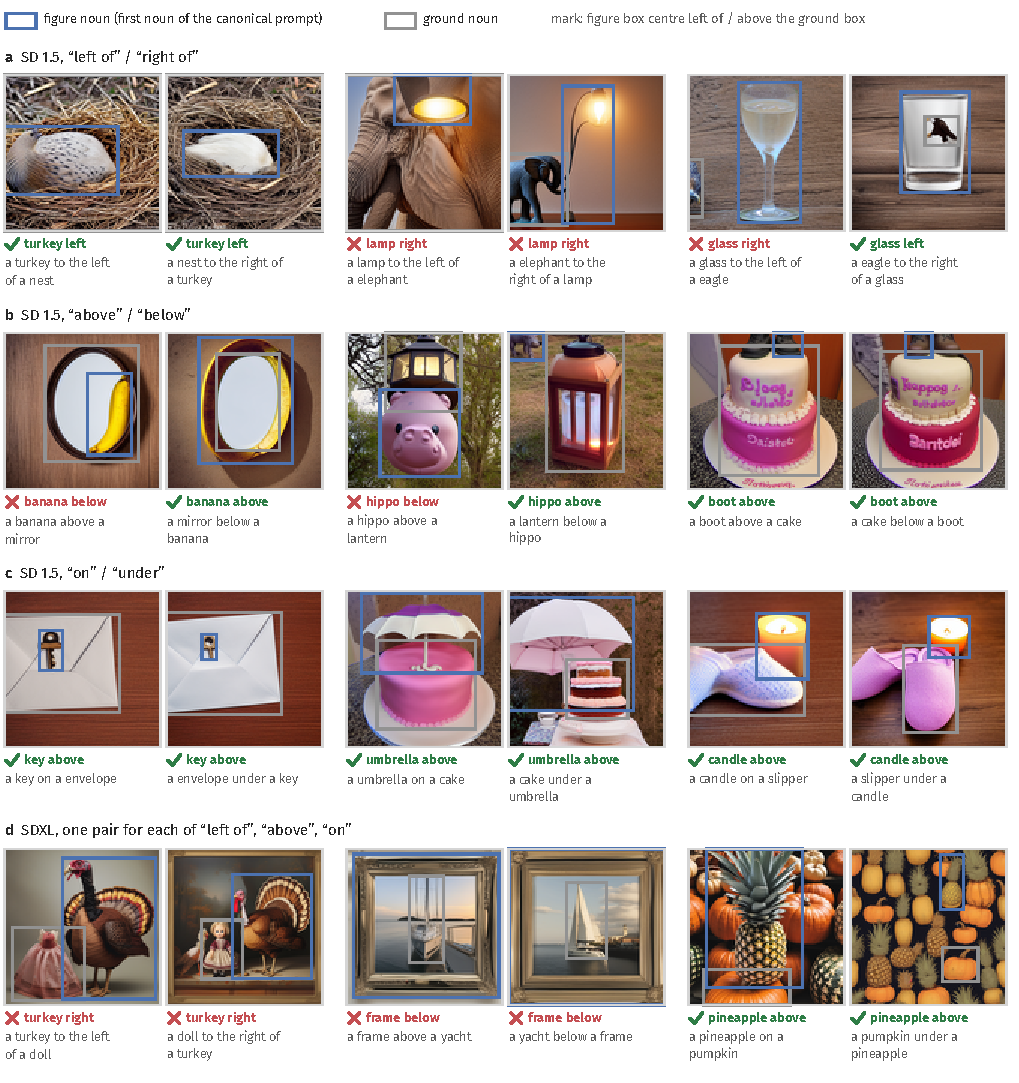
\includegraphics[width=\linewidth]{fig_case_generation.pdf}
  \caption{\textbf{Generated layouts ignore the relation word.} Each pair shows one prompt and its converse under the same seed (seed 0), with the detected boxes of the figure noun (blue) and the ground noun (grey), and a mark when the figure's box centre lies left of or above the ground's. The pairs are the first in index order, three per relation for SD 1.5 and one per relation for SDXL, whose two phrasings both hold both objects at the detection threshold of Section~\ref{sec:diffusion}. Prompts appear verbatim from the template, which writes ``a'' before every noun.}
  \label{fig:case_generation}
\end{figure}

Figure~\ref{fig:case_generation} shows the kinds of failure behind the rates of Section~\ref{sec:diffusion}. The lamp and the elephant keep one layout under both phrasings of \textsc{left of}, so the figure lands on the wrong side twice, while the turkey lands on the left of the nest under both phrasings. In three SD 1.5 pairs, the glass and the eagle, the banana and the mirror, and the hippo and the lantern, the figure lands in its place under one phrasing and out of it under the other, which a model that read the relation would avoid. Every \textsc{on} pair puts the figure on top in both phrasings, as stacking one object on the other would, and SDXL keeps the turkey and the frame on the wrong side in both phrasings and tiles the canvas with pumpkins in the converse of the last pair.

\begin{figure}[!htbp]
  \centering
  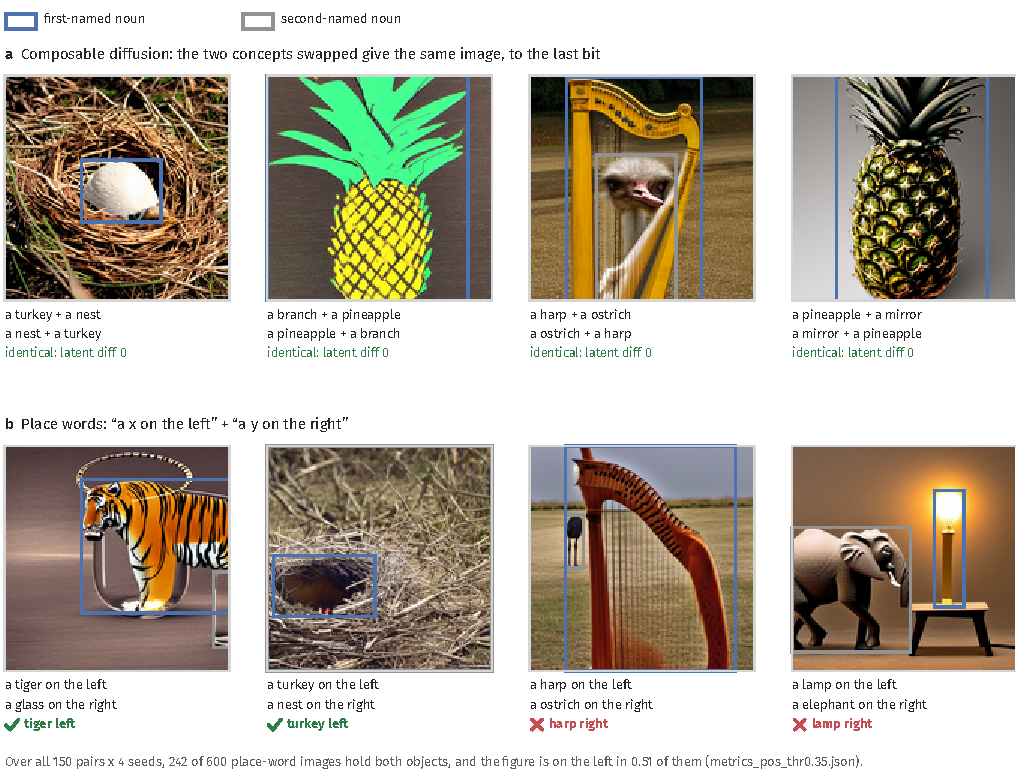
\includegraphics[width=\linewidth]{fig_case_compose.pdf}
  \caption{\textbf{Composable diffusion marks no roles, and place words do not fix one.} \textbf{a.} The first four pairs of the swap check: adding the two concepts' scores in either order gives the same latent to the last bit. \textbf{b.} Place words in each concept's prompt. The tiger pair comes from the main text, and the other three are the first pairs in index order with both objects detected at seed 0; the mark tells whether the figure sits on the left.}
  \label{fig:case_compose}
\end{figure}

Figure~\ref{fig:case_compose}a shows the symmetry of composable diffusion directly. Each swapped pair gives one image, because a sum of scores is the same in either order, so any role in the scene must come from the wording of each prompt. Place words supply such a wording, and Figure~\ref{fig:case_compose}b shows them succeeding for the tiger and the turkey and failing for the harp and the lamp. Over all 600 place-word images, 242 hold both objects, and the figure sits on the left in 0.51 of those.

\FloatBarrier
\subsection{Image Encoders}
\label{app:case_places}

\begin{figure}[!htbp]
  \centering
  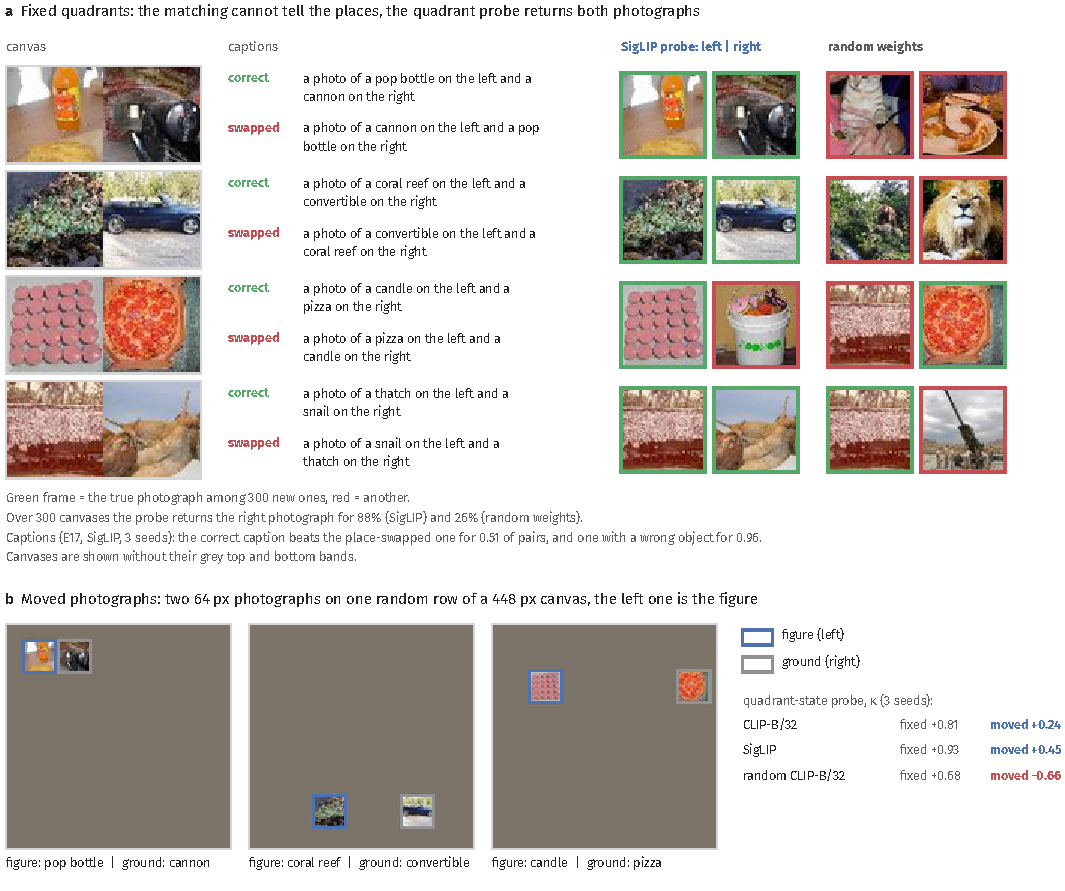
\includegraphics[width=\linewidth]{fig_case_places.pdf}
  \caption{\textbf{Image encoders keep fixed places that their matching ignores, and moving the photographs removes most of them.} \textbf{a.} The first four pairs of new photographs with named classes, each on a fixed-quadrant canvas, with the correct and the place-swapped caption, and the photographs that the linear probe of SigLIP's quadrant states returns for the left and the right role (green when correct among 300 new photographs), beside the same probe of a random-weight copy. \textbf{b.} The first three pairs placed as in the moved-photograph test of Section~\ref{sec:images}, where the left photograph is the figure, with $\kappa$ of the quadrant-average probe under fixed and moved placement (3 seeds).}
  \label{fig:case_places}
\end{figure}

In Figure~\ref{fig:case_places}a, SigLIP's caption matching prefers the correct caption over the place-swapped one on 0.51 of pairs, while its quadrant probe returns the right photograph in seven of the eight places shown and in 88\% of 300 canvases. The probe misses only the pizza, for which it returns a bucket. The random-weight copy returns the right photograph in two of the eight places and in 26\% of canvases. The moved canvases of Figure~\ref{fig:case_places}b show why the fixed quadrants overstate the role code. Two small photographs on one row can sit anywhere, so a place in the state no longer names a role, and $\kappa$ falls from 0.81 to 0.24 for CLIP-B/32 and from 0.93 to 0.45 for SigLIP.

\FloatBarrier
\subsection{Language Models}
\label{app:case_lm}

\begin{figure}[!htbp]
  \centering
  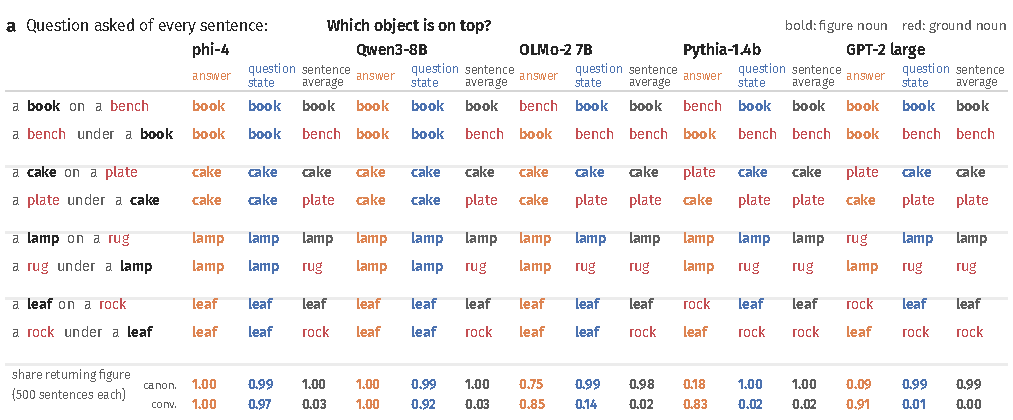
\includegraphics[width=\linewidth]{fig_case_lm.pdf}
  \caption{\textbf{Answers and states for four sentence pairs in five models.} The first four saved pairs of the relation \emph{on}/\emph{under}, each in its canonical and its converse phrasing, under the question ``Which object is on top?''. For each model, the answer (orange when it names the figure, red when it names the ground), the noun returned by the figure probe of the question state (blue when correct, red otherwise) and the noun returned by the same probe of the token-averaged sentence state (grey when correct, red otherwise). The bottom rows give the share returning the figure over 500 sentences of each phrasing.}
  \label{fig:case_lm}
\end{figure}

Figure~\ref{fig:case_lm} follows four sentence pairs through five models. phi-4 and Qwen3-8B name the figure in all eight sentences, and the figure probe of their question state returns the figure in all eight as well. Pythia-1.4b and GPT-2 large name the second-mentioned noun in seven of eight sentences, \emph{plate} for ``a cake on a plate'' and \emph{cake} for ``a plate under a cake'', and the probe of their question state returns the first-mentioned noun in every sentence, so answer and state both follow word order, from opposite ends of the sentence. OLMo-2 7B answers by meaning in seven of eight sentences, while its question-state probe returns the ground in three of the four converse sentences, the gap that Section~\ref{sec:behavior} traces to a role code that our linear probes miss. In every model, the probe of the token-averaged sentence state returns the first-mentioned noun, which is the figure in canonical sentences and the ground in converse ones.

\FloatBarrier
\subsection{Glyph Networks}
\label{app:case_glyph}

\begin{figure}[!htbp]
  \centering
  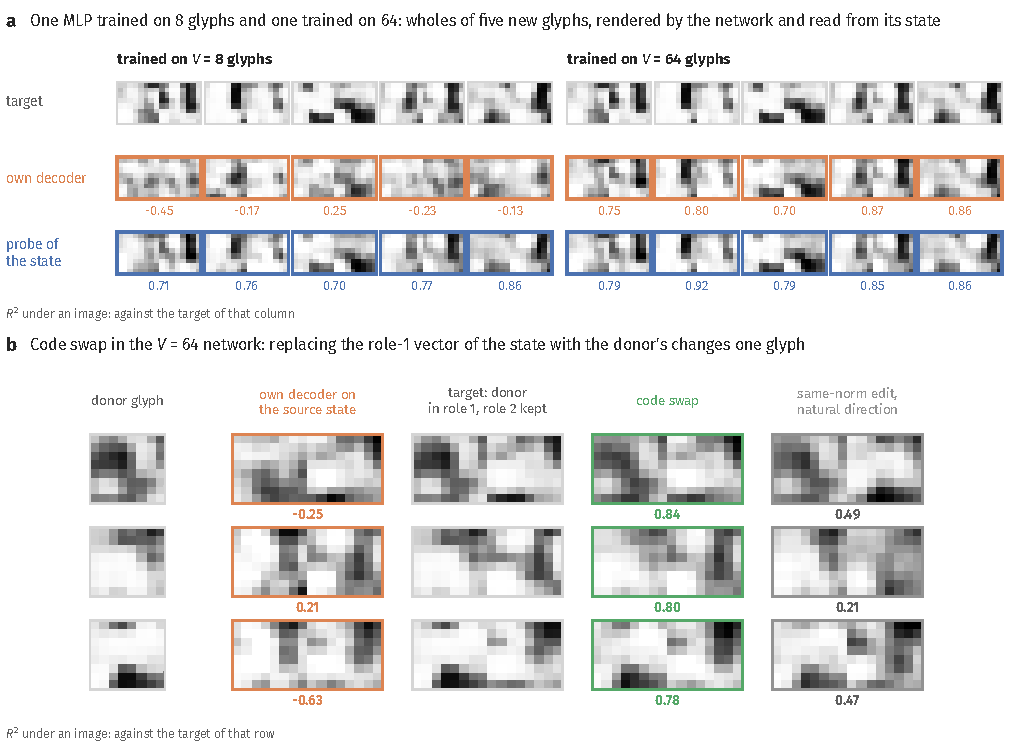
\includegraphics[width=\linewidth]{fig_case_glyph.pdf}
  \caption{\textbf{Glyph networks keep new glyphs their decoders cannot draw, and their decoders read the role codes.} \textbf{a.} Every saved whole of new glyphs for one MLP trained on 8 glyphs and one trained on 64 ($m = 64$, \textsc{over}, seed 0): the target, the network's own decoder and a linear probe of its state, with $R^2$ against each target. \textbf{b.} All three saved code swaps in the 64-glyph network: the donor glyph, the decoder on the source state, the target with the donor in role 1, the decoder after the code swap, and an edit of the same norm along the natural direction $h(a', b') - h(a, b)$, with $R^2$ against the target.}
  \label{fig:case_glyph}
\end{figure}

In Figure~\ref{fig:case_glyph}a, the decoder of the 8-glyph network misses most of each new glyph, with $R^2$ between $-0.45$ and 0.25, while a linear probe of the same state reconstructs each whole at 0.70--0.86. With 64 training glyphs the decoder catches up, at 0.70--0.87, and the probe stays at 0.79--0.92. In Figure~\ref{fig:case_glyph}b, writing a donor's vector into role 1 makes the decoder draw the donor in role 1 and keep the role-2 glyph, at 0.78--0.84 against the target, while an edit of the same norm along the natural direction reaches 0.21--0.49.
\FloatBarrier
